\documentclass[conference]{IEEEtran} % Clase IEEEtran para formato IEEE
\usepackage[utf8]{inputenc} % Codificación de caracteres
\usepackage[spanish]{babel} % Idioma español
\usepackage{amsmath, amssymb} % Paquetes para matemáticas
\usepackage{graphicx} % Paquete para incluir imágenes
\usepackage{cite} % Paquete para gestionar referencias
\usepackage{hyperref} % Paquete para hipervínculos
\usepackage{float} % Para forzar la posición de figuras


\title{Smart SSH Terminal} 
\author{
    \IEEEauthorblockN{Andres Felipe Gonzalez Garzon, Haider Andres Cañon Murcia}
    \IEEEauthorblockA{
        Bogotá, Colombia \\ 
        \texttt{andres-gonzalez16@upc.edu.co, Haider-canon@upc.edu.co} % [cite: 2]
    }
}

\begin{document}


\maketitle


\begin{abstract}
A lo largo de la historia de internet, los sistemas operativos han jugado 
un papel fundamental. En particular, los sistemas basados en Unix,
como Linux, constituyen la columna vertebral de la infraestructura que sostiene la red global.
Su administración se realiza principalmente a través de la terminal de línea de comandos. Este paper
propone una solución innovadora que integra un modelo de lenguaje grande (LLM) en un cliente SSH, 
facilitando la interacción y el aprendizaje en el entorno de la terminal.
\end{abstract}


\begin{IEEEkeywords}
SSH, Linux, LLM, Terminal Inteligente, cliente SSH, Administración de Sistemas, Asistente de IA, Unix/Linux
\end{IEEEkeywords}


\section{Introducción}
Desde los orígenes de la computación moderna, los sistemas operativos han 
sido el puente entre el ser humano y la máquina. Sin importar la época ni 
el fabricante, todos ellos han compartido un rasgo común: una interfaz de 
comandos textual que, si bien otorga un control preciso y profundo sobre el 
sistema, exige al usuario memorizar una sintaxis extensa, interpretar 
mensajes de error crípticos y construir mentalmente un modelo abstracto de 
cómo funciona el sistema \cite{shneiderman1982future}. Este escenario, que 
décadas atrás era exclusivo de especialistas, sigue siendo hoy el punto de 
entrada obligado para cualquier persona que aspire a comprender y gestionar 
sistemas operativos basados en Unix/Linux \cite{ritchie1974unix}. El 
resultado es documentado empíricamente: los mensajes de error de las 
herramientas de línea de comandos presentan una dificultad sustancial para 
los usuarios novatos \cite{becker2019compiler}; esta dificultad desencadena 
ciclos de frustración \cite{ossovski2024frustration} que, si se repiten sin 
retroalimentación efectiva, producen desenganche emocional progresivo de la 
tarea —patrón documentado en novatos de programación ante errores repetidos 
 \cite{bosch2017affective} y estructuralmente análogo al aprendizaje de 
entornos CLI, donde la misma ausencia de retroalimentación inmediata opera 
como factor de abandono. 

El auge reciente de los Modelos de Lenguaje Grande (LLMs) representa un 
punto de inflexión en este panorama. Por primera vez, es posible interactuar 
con sistemas complejos empleando lenguaje natural, recibir explicaciones 
contextuales al instante y obtener asistencia en la resolución de errores 
sin abandonar el entorno de trabajo \cite{brown2020language, chen2021evaluating}. 
Esta capacidad abre una oportunidad sin precedentes para transformar la 
forma en que los estudiantes y técnicos aprenden a operar un sistema 
operativo: no a través de la memorización pasiva, sino mediante la práctica 
guiada, contextual y progresiva \cite{denny2023conversing}. Sin embargo, en 
la práctica actual, la asistencia de IA permanece desacoplada del entorno 
donde ocurre el aprendizaje: el estudiante interrumpe su sesión de terminal, 
consulta un chatbot en el navegador y regresa al contexto de trabajo habiendo 
perdido tanto el flujo cognitivo como la trazabilidad del error. Para que el 
potencial pedagógico de los LLMs se materialice, la inteligencia artificial 
debe integrarse de forma nativa en el mismo espacio donde ocurre la 
práctica: la terminal remota. 

Precisamente de esa necesidad nace \textit{Smart SSH Terminal}: un entorno 
de trabajo integrado que fusiona en una sola interfaz el acceso remoto 
seguro vía SSH, la gestión de archivos por SFTP y un asistente de IA 
contextual que acompaña al usuario en tiempo real. La herramienta está 
dirigida tanto a estudiantes de ingeniería como a técnicos en formación que 
requieren un andamiaje inteligente para desarrollar competencias reales en 
el manejo de Linux en entornos de laboratorio remoto con recursos limitados. 
Estos requisitos de eficiencia de memoria, bajo consumo de CPU y seguridad 
en las comunicaciones motivaron la elección de Rust y el framework Tauri 
como base tecnológica \cite{klabnik2019rust}. 

Las soluciones existentes abordan estos problemas de forma parcial: los 
clientes SSH tradicionales carecen de componente pedagógico; las plataformas 
de aprendizaje interactivo de Linux no ofrecen acceso real a infraestructura 
remota; y los terminales modernos con IA como Warp presentan limitaciones 
funcionales sobre sesiones SSH remotas y no incorporan mecanismos de 
andamiaje progresivo \cite{warp2024ssh}. Ninguna herramienta integra 
simultáneamente acceso remoto autenticado, gestión de archivos y asistencia 
de IA pedagógica contextual en un único entorno. La Sección~II documenta 
este vacío en detalle. 

Las contribuciones principales de este trabajo son: (1) el diseño e 
implementación de \textit{Smart SSH Terminal}, un cliente SSH con asistente 
de IA integrado de forma nativa que transforma los errores de ejecución en 
retroalimentación pedagógica contextual; (2) una arquitectura eficiente en 
Rust y Tauri que satisface los requisitos de cómputo de servidores de 
laboratorio de bajo coste; y (3) una evaluación empírica del sistema sobre 
infraestructura real, con métricas de rendimiento (uso de CPU, memoria y 
latencia de respuesta). 

El resto del artículo se organiza así: la Sección~II revisa los trabajos 
relacionados; la Sección~III describe la arquitectura del sistema y sus 
subsistemas; la Sección~IV justifica las decisiones de implementación, en 
 particular la adopción de Rust; la Sección~V presenta la metodología de 
pruebas y los resultados en el laboratorio remoto; finalmente, las 
Secciones~VI y VII abordan el trabajo futuro y las conclusiones.

\section{Diseño Arquitectónico}

\subsection{Arquitectura General: Topología de Red y Capas Lógicas}

En un enfoque alineado con las arquitecturas de software modernas, el sistema ha sido concebido bajo un modelo encapsulado en el que la totalidad del aplicativo reside en la estación de usuario (Smart Client). Este diseño exime la necesidad de desplegar servidores propietarios intermedios; en su lugar, la lógica recae sobre una aplicación cliente autónoma que se acopla directamente a entidades externas y estandarizadas (como placas de desarrollo IoT o servidores Linux corporativos).

Como se ilustra en la Figura~\ref{fig:arquitectura_general}, la topología global describe una única \textbf{Aplicación Local} que emplea protocolos seguros para orquestar la interacción técnica con: (1) el \textbf{Laboratorio Físico} (ej. dispositivos Raspberry Pi mediante servicios nativos), (2) \textbf{Servicios Semánticos} (Plataformas LLM en la nube o locales) y (3) Servicios de Directorio Institucional (\textbf{LDAP}).

\begin{figure}[ht]
    \centering
    \includegraphics[width=\linewidth]{images/arquitectura_general.png}
    \caption{Topología general del sistema que demuestra la autonomía de la aplicación local frente a integraciones externas, prescindiendo de servidores intermediarios propios.}
    \label{fig:arquitectura_general}
\end{figure}

A nivel interno, la aplicación cliente se divide en tres capas lógicas fundamentales comunicadas asíncronamente mediante un canal de paso de mensajes (IPC, de sus siglas en inglés), lo cual garantiza alta resiliencia y el aislamiento de las operaciones de red.

\subsubsection{Capa de Presentación e Interacción}
Representa la superficie de control de cara al usuario. Su objetivo es unificar múltiples canales de administración remota de forma visual y reactiva (ver Figura~\ref{fig:subsistema_presentacion}). Esta capa se compone de módulos funcionales interdependientes que operan bajo un gestor de estado centralizado:
\begin{itemize}
    \item \textbf{Emulador de Terminal}: Procesa el flujo estándar de entrada y salida (I/O) emulando secuencias de control para soportar interactividad basada en texto de alta densidad.
    \item \textbf{Explorador de Archivos y Paneles de Control}: Traducción gráfica que transforma acciones de alto nivel (como clicks sobre visores VNC) en operaciones de red directas al flujo del sistema operativo remoto.
    \item \textbf{Interfaz de Asistencia Conversacional}: Elemento de retroalimentación pedagógica, que sincroniza su contenido bidireccionalmente con las salidas de error o bloqueos presentados en el emulador de terminal.
\end{itemize}

\begin{figure}[ht]
    \centering
    \includegraphics[width=\linewidth]{images/subsistema_presentacion.png}
    \caption{Diagrama estructural de la Capa de Presentación e Interacción.}
    \label{fig:subsistema_presentacion}
\end{figure}

\subsubsection{Capa de Procesamiento y Control (Core)}
Actúa como el motor de red y de sesión en el que se delegan las operaciones críticas. Como se indica en la Figura~\ref{fig:subsistema_nucleo}, esta capa administra los algoritmos criptográficos, protocolos robustos de transporte y la auditoría de uso:
\begin{itemize}
    \item \textbf{Motor de Canal Seguro}: Implementa el estándar SSH y sus negociaciones seguras (cifrado asimétrico), operando sobre descriptores para mantener multiplexados de forma asíncrona un túnel de terminal y flujos de red.
    \item \textbf{Motor de Transferencia de Archivos}: Encargado de empaquetar, enrutar y desempaquetar ráfagas binarias hacia el daemon SFTP o equivalentemente integrado en la conectividad del laboratorio remoto.
    \item \textbf{Orquestador de Trazabilidad}: Mecanismo que captura heurísticamente trazas de ejecución en la sesión, brindando al sistema una bitácora altamente estructurada de cada paso del operario.
\end{itemize}

\begin{figure}[ht]
    \centering
    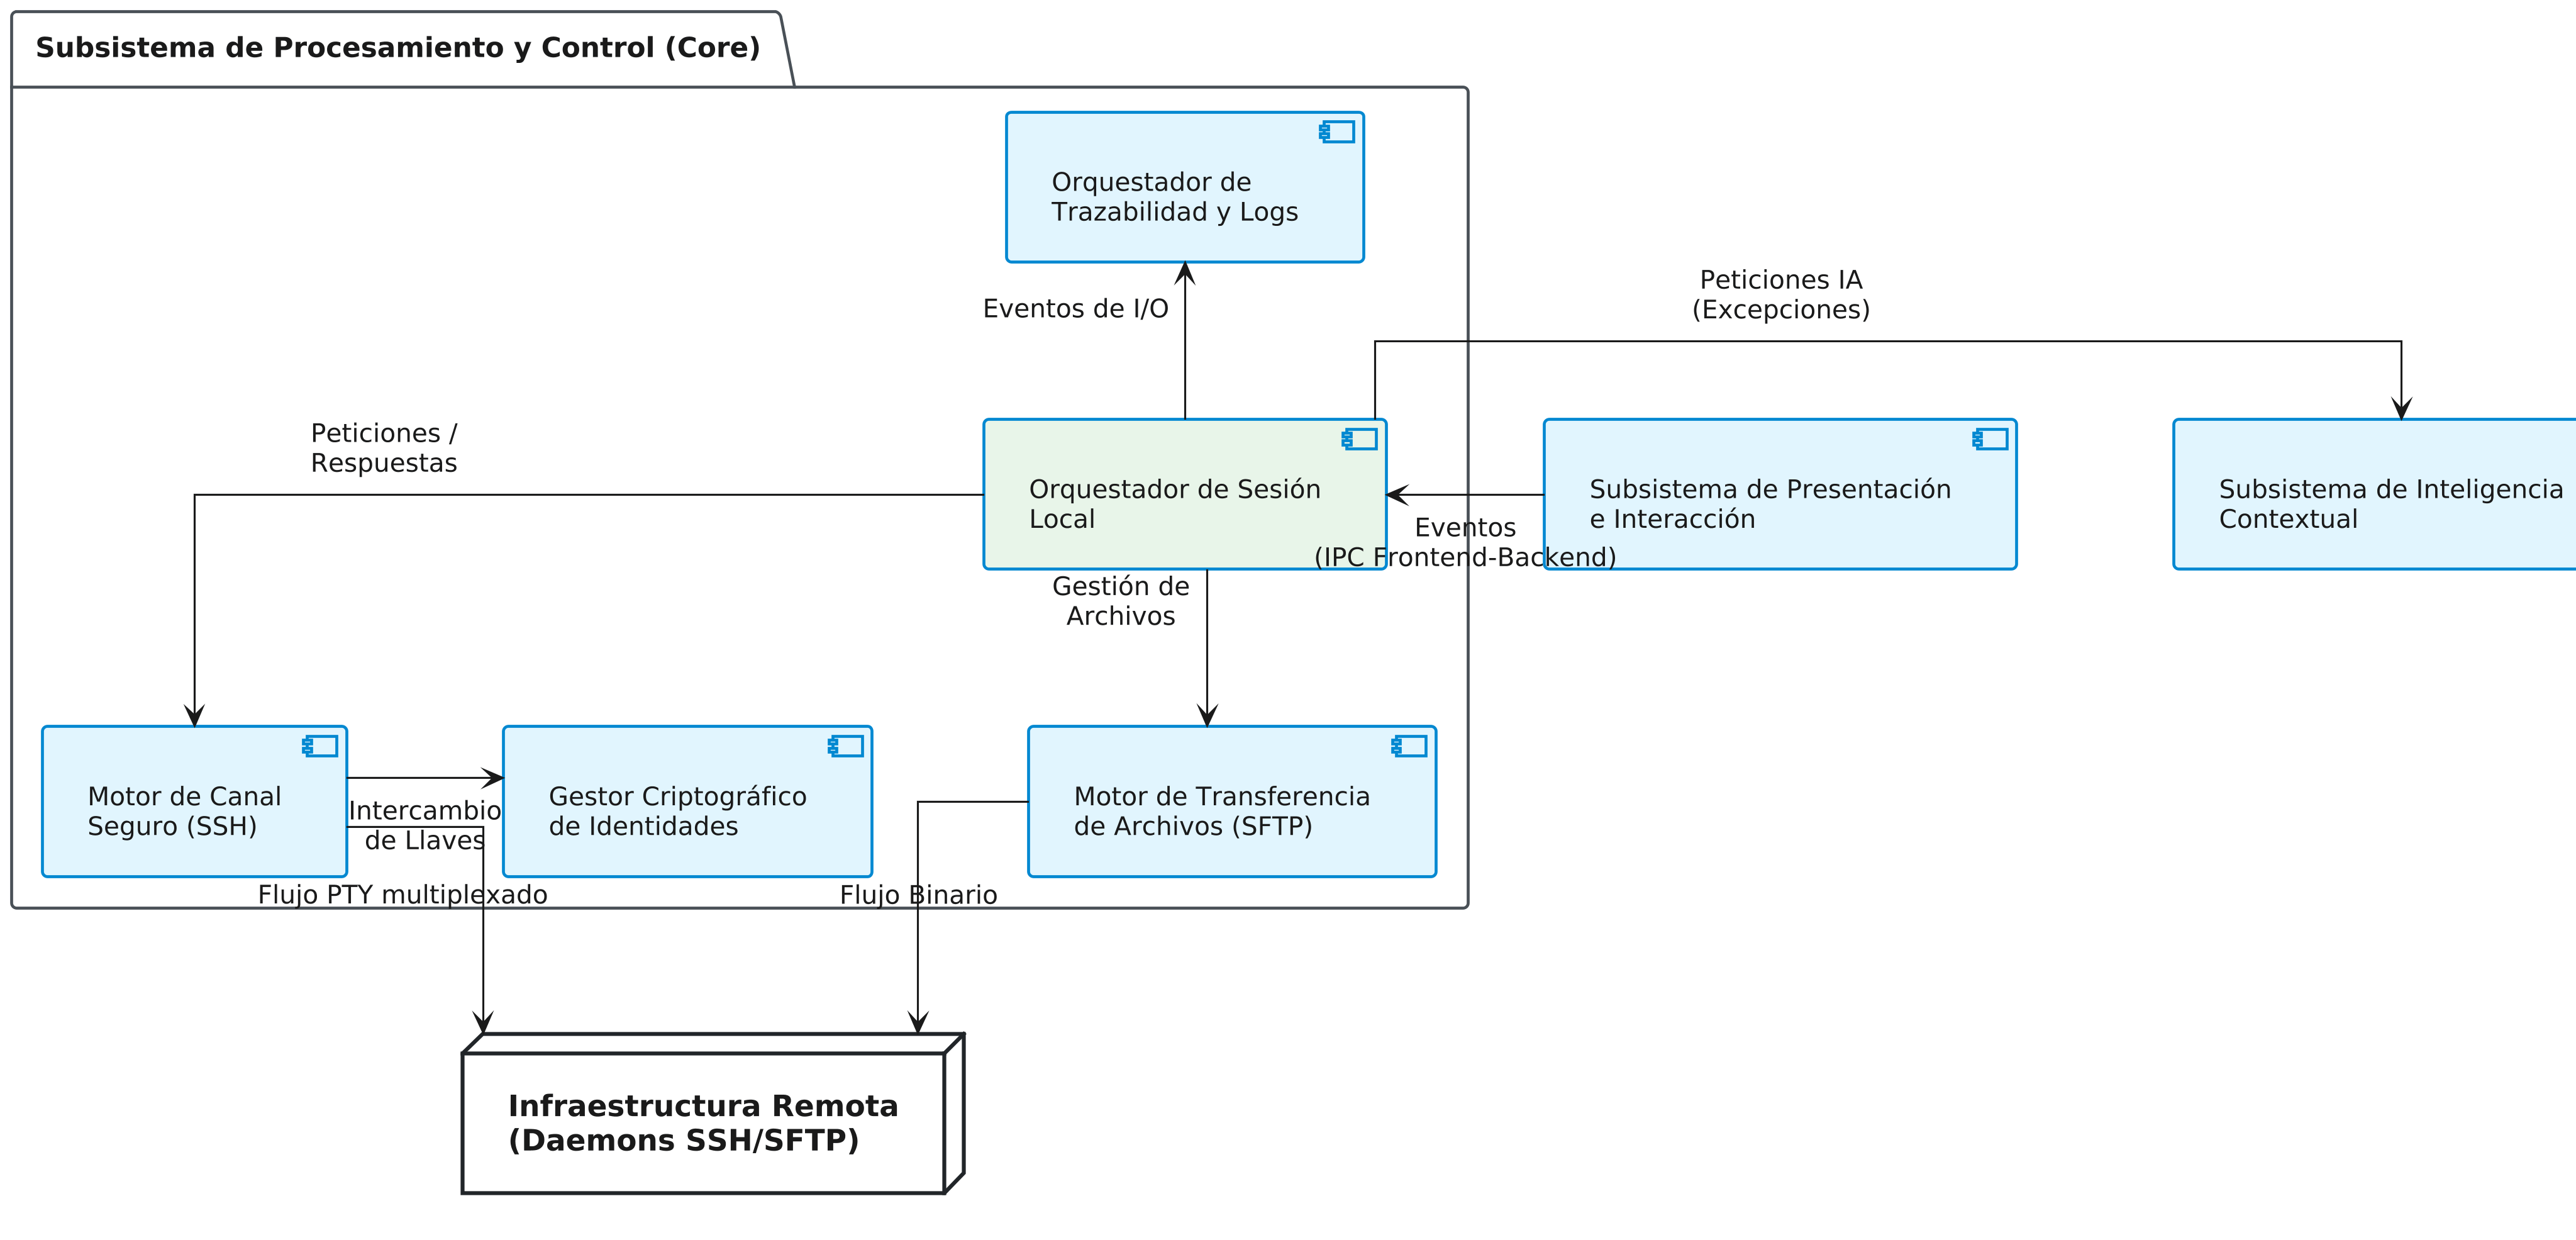
\includegraphics[width=\linewidth]{images/subsistema_nucleo.png}
    \caption{Módulos transaccionales y de conectividad de la Capa de Procesamiento Interno.}
    \label{fig:subsistema_nucleo}
\end{figure}

\subsubsection{Capa de Inteligencia Artificial Contextual}
Esta capa, ilustrada en la Figura~\ref{fig:subsistema_agente}, funge como puente middleware entre la estación cliente local y la red de transformadores y LLMs proveedores de respuestas, habilitando las capacidades de andamiaje:

\begin{itemize}
    \item \textbf{Descubrimiento de Recursos (Context Protocol)}: Dotación técnica que rompe el paradigma aislado de los chatbots, permitiendo a la IA inspeccionar el estado actual (archivos, logs del host remoto) como suplemento antes de retornar respuestas y deduciendo así el estado exacto del entorno con extrema fidelidad técnica.
    \item \textbf{Construcción de Contexto Pragmático}: Submodulo que enhebra un grafo con las salidas de error previas y con los comandos que generaron dichas anomalías de red o fallo general.
    \item \textbf{Motor Lógico de Prácticas Guiadas}: Autómata evaluador que sincroniza las habilidades demostradas en los comandos de sesión con escenarios metodológicos pautados de laboratorio (fases), personalizando la ayuda a la meta de aprendizaje.
\end{itemize}

\begin{figure}[ht]
    \centering
    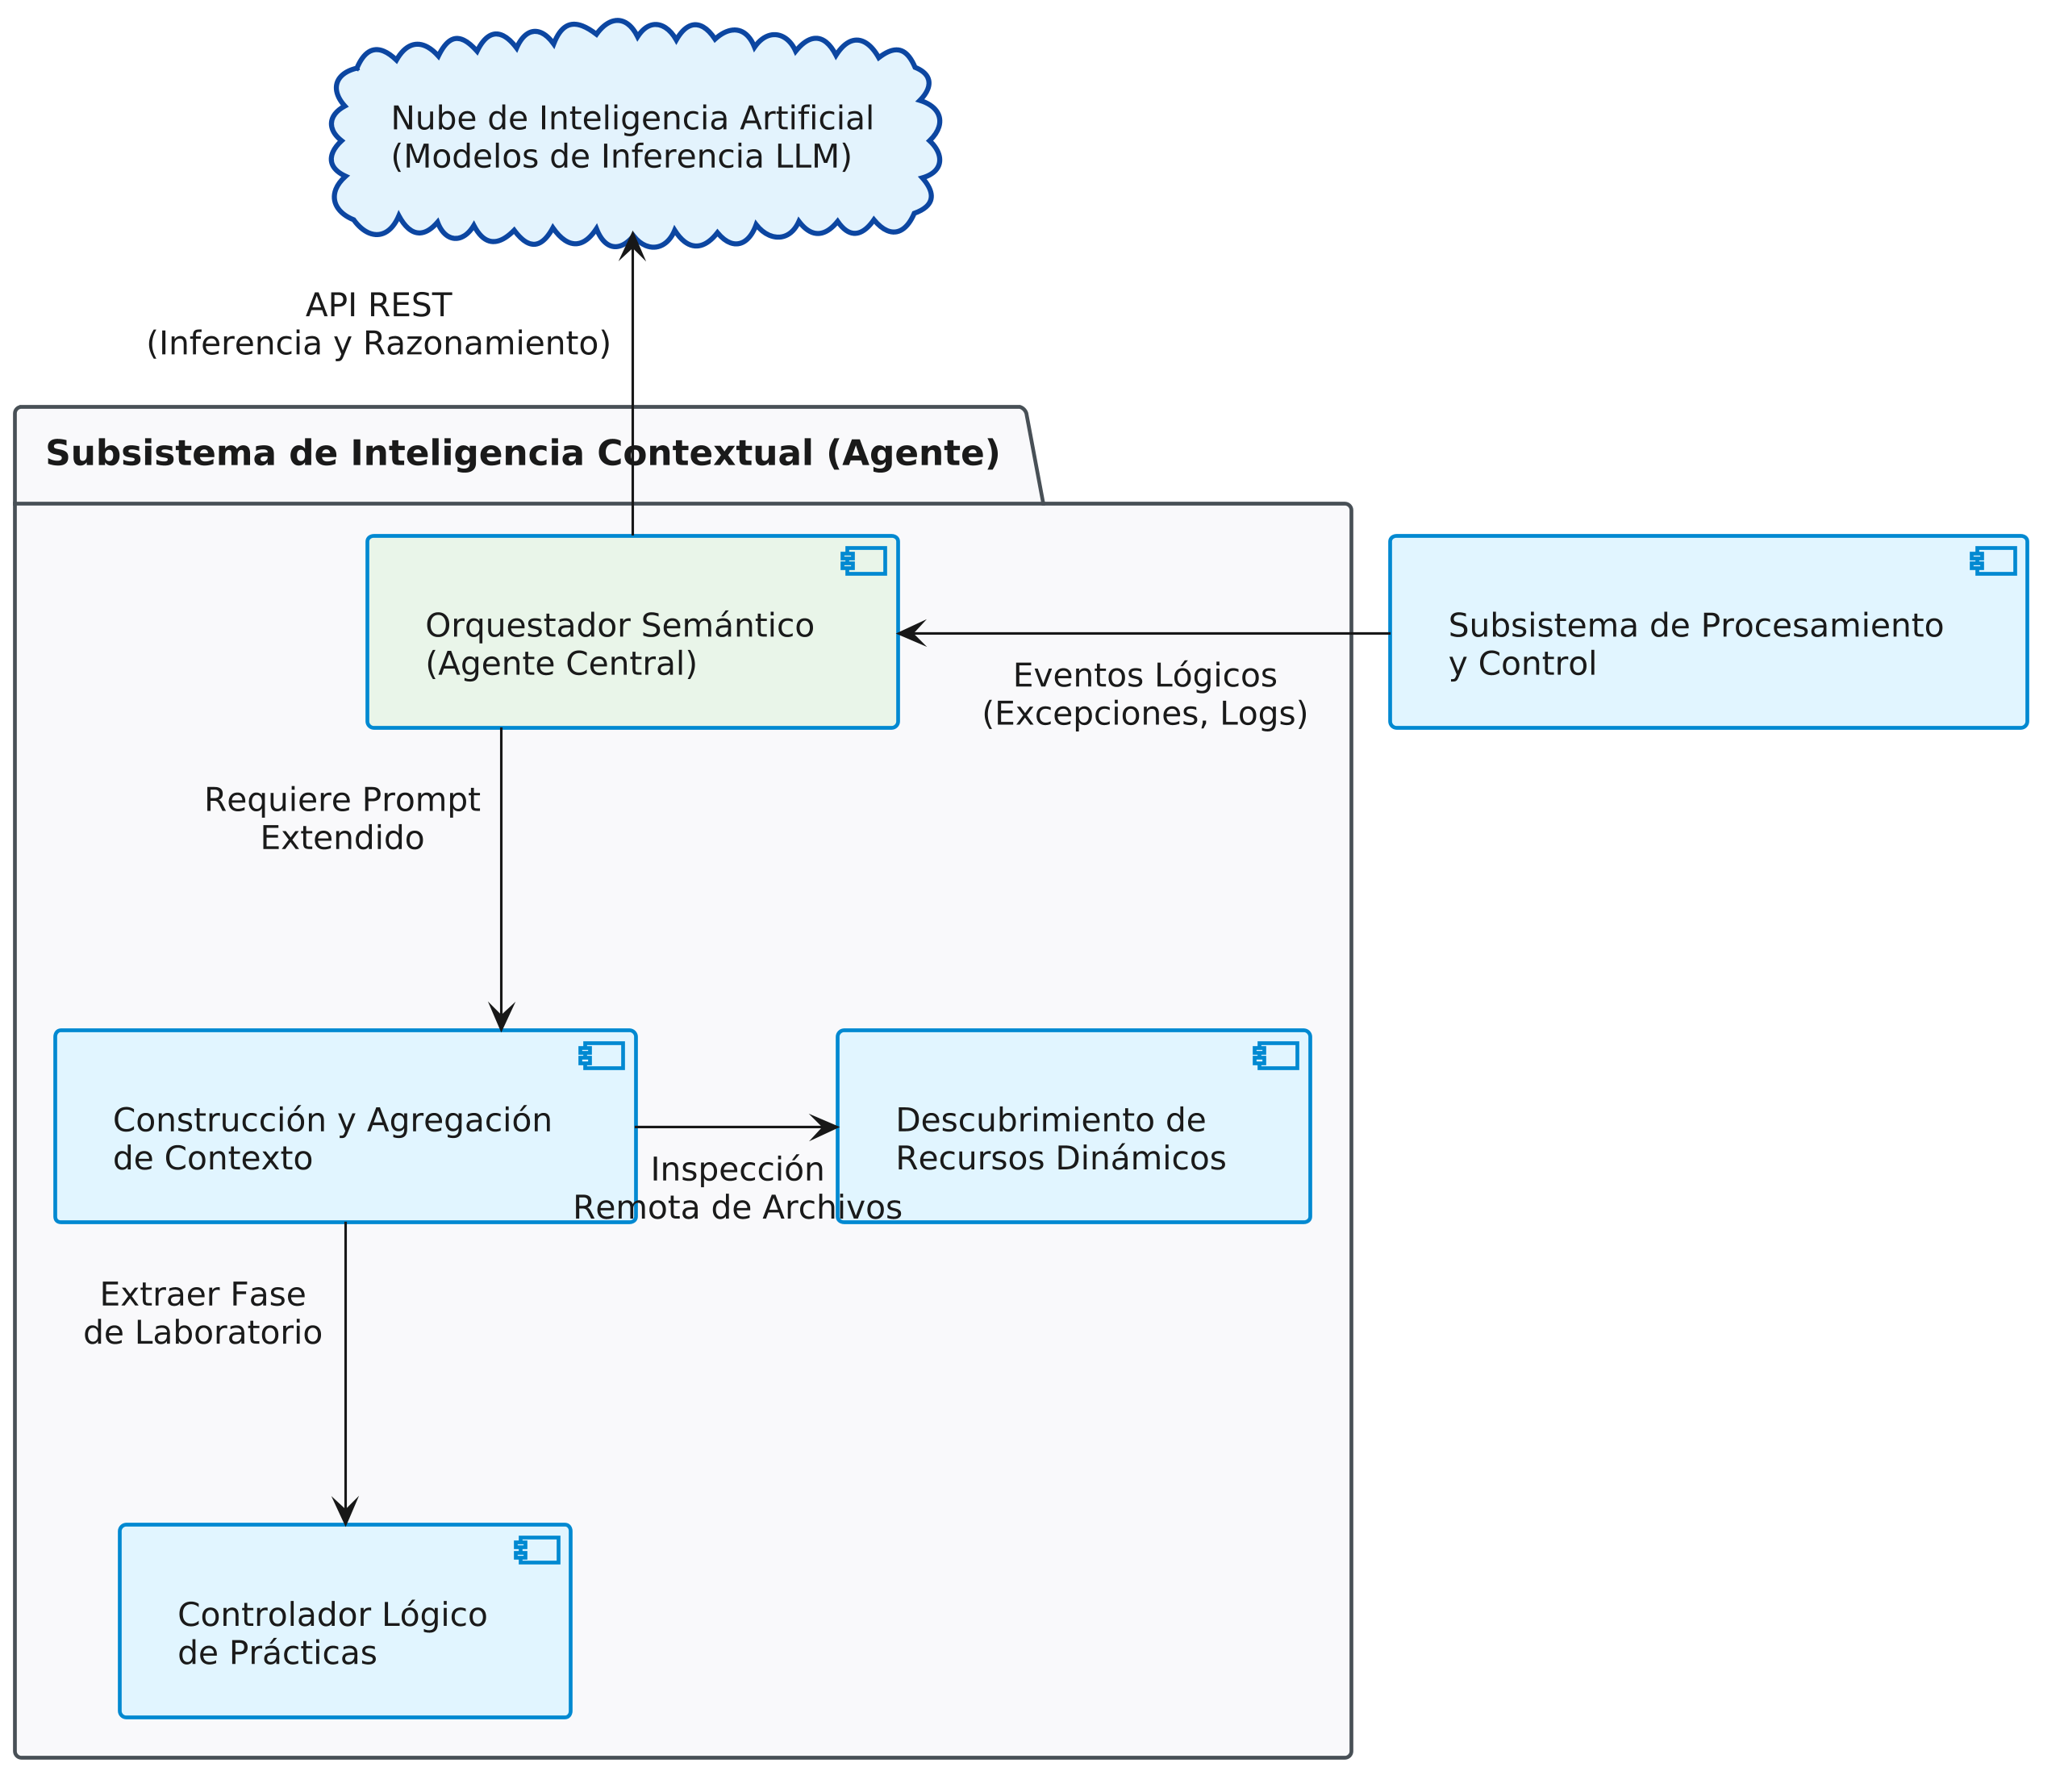
\includegraphics[width=\linewidth]{images/subsistema_agente.png}
    \caption{Capa Semántica responsable de la coordinación de contexto hacia endpoints LLM.}
    \label{fig:subsistema_agente}
\end{figure}

\subsection{Integración Arquitectónica y Beneficios Subyacentes}

La topología expuesta erradica la fragmentación típica encontrada en clientes remotos \cite{mobaxterm_misc}. La consolidación de canales (como conexiones SSH reusadas y WebSockets noVNC para escritorios virtuales) fusionados con un servicio \textit{endpoint} inteligente reduce de forma abismal la latencia cognitiva de transición. El estudiante experimenta un \textit{sandbox} único en donde errores operacionales son inmediatamente atrapados y digeridos semánticamente para proponer un apoyo educativo ininterrumpido.

\section{Implementación}
\subsection{Evolución del desarrollo}
El desarrollo de esta herramienta comenzó inicialmente utilizando Tkinter, debido a que representaba la vía más rápida para prototipar una interfaz gráfica básica. Sin embargo, durante esta etapa se identificaron problemas críticos relacionados con el refresco de pantalla y la fluidez necesaria para un emulador de terminal en tiempo real.

\subsection{Justificación de Rust}
Ante las limitaciones de rendimiento encontradas, se decidió realizar un salto tecnológico hacia Rust \cite{klabnik2019rust}. Este lenguaje fue elegido por su enfoque en la seguridad de memoria \cite{jung2017rustbelt}, su alto rendimiento comparable al de C/C++ \cite{levy2017rust}, y su ecosistema moderno que facilita la creación de aplicaciones de escritorio seguras. Rust permite una gestión eficiente de hilos y una respuesta inmediata en la interfaz de usuario.

\subsection{Integración de servicios}
La aplicación actual ya incorpora servicios equivalentes a los ofrecidos por herramientas tradicionales como WinSCP \cite{mobaxterm_misc}, permitiendo la gestión gráfica de archivos mediante el protocolo SFTP de forma integrada con la terminal.

\subsection{La Novedad}
La principal innovación radica en haber logrado una interfaz limpia y amigable que no solo emula una terminal, sino que es capaz de realizar un seguimiento inteligente a las acciones del usuario, ofreciendo asistencia contextual proactiva sin sobrecargar la experiencia de uso.

\section{Escenario de Pruebas}
\label{sec:pruebas}
\subsection{Metodología}
Para validar la herramienta, se llevó a cabo una metodología de pruebas con un grupo de 10 personas con distintos niveles de experiencia en Linux. El objetivo fue evaluar la facilidad de uso y la efectividad de la asistencia por IA.

\subsection{Métricas y gráficas}
Los resultados mostraron tiempos de uso promedio de 20 minutos de interacción continua, durante los cuales los usuarios lograron generar comandos complejos y realizar tareas de administración que normalmente requerirían consultas externas a la documentación.

\subsection{Laboratorio remoto}
La interfaz permite acoplarse a un escenario de laboratorio remoto \cite{garcia2010web}, como el uso de una Raspberry Pi \cite{de2011virlab}. Esto permite a los usuarios desarrollar prácticas reales mientras monitorean el entorno físico. A continuación se presentan fotografías de evidencia del funcionamiento en este entorno.

\begin{figure}[H]
    \centering
    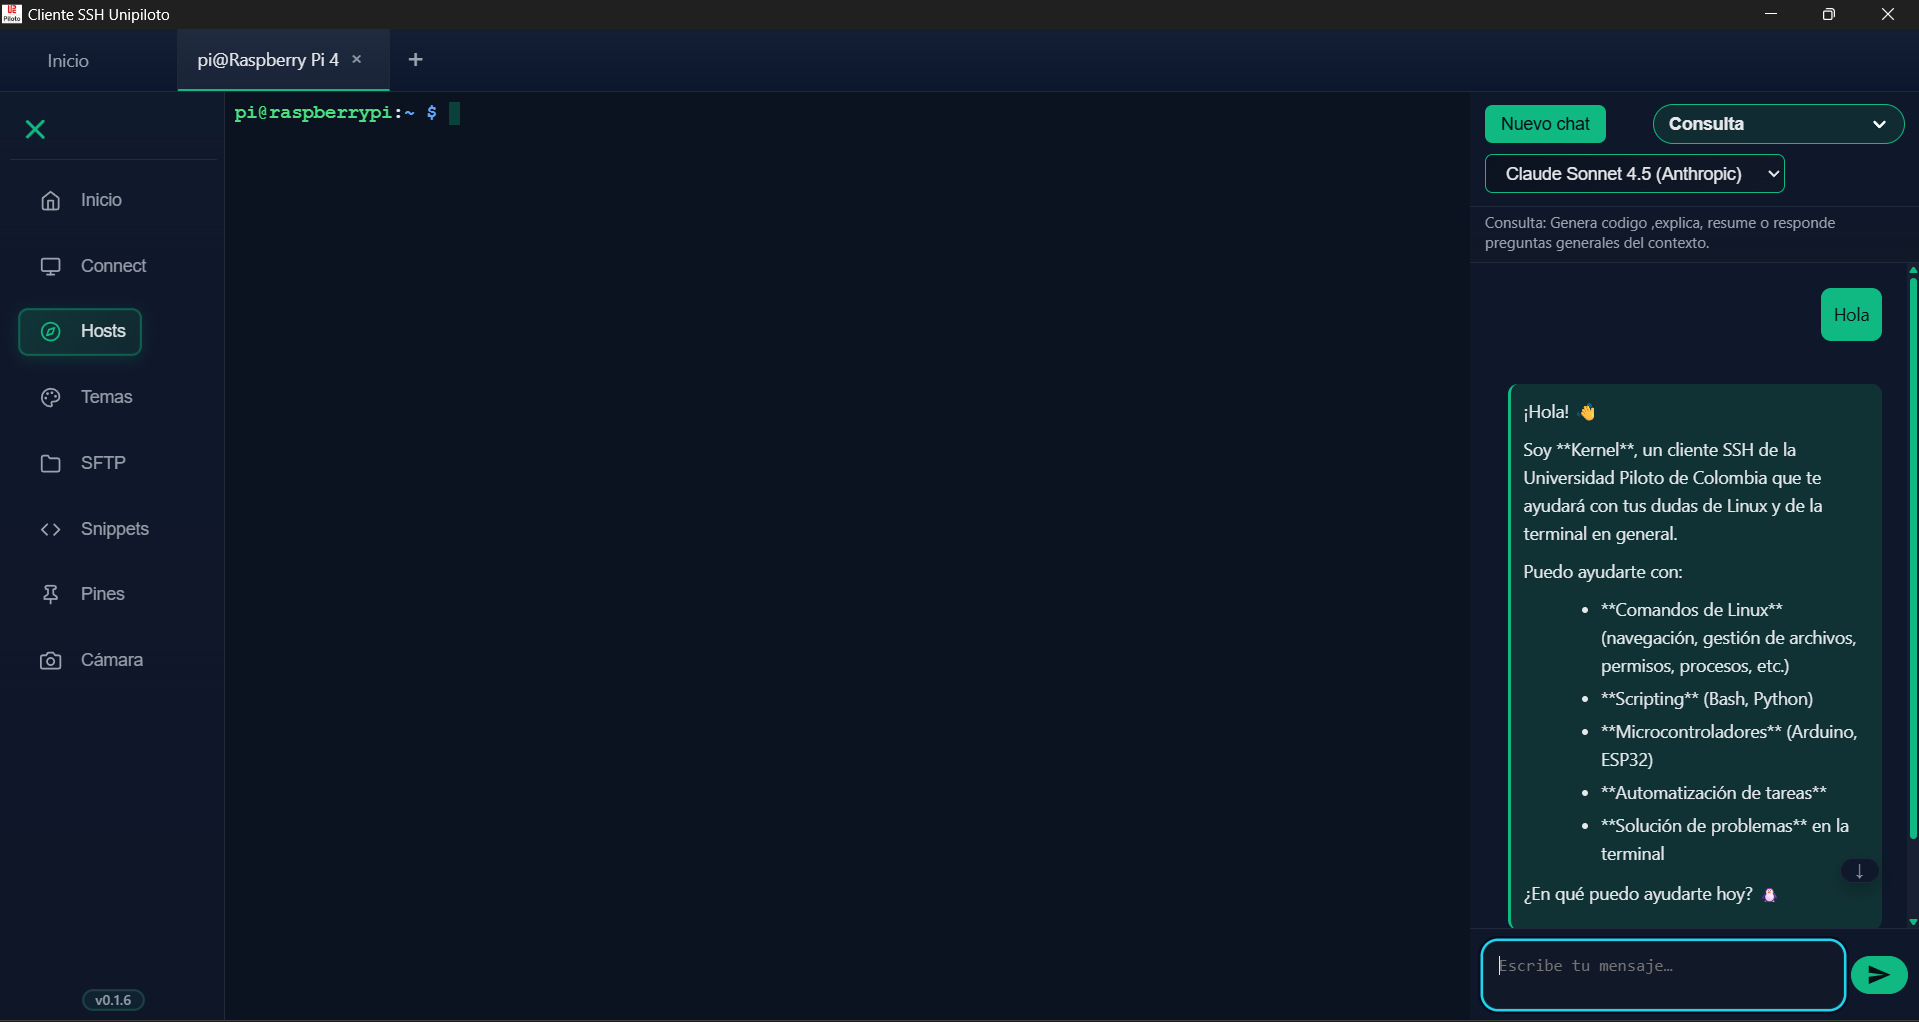
\includegraphics[width=\linewidth]{images/VistasoPrograma.png}
    \caption{Interfaz del programa en ejecución.}
    \label{fig:vistaso}
\end{figure}

\section{Trabajo Futuro}
Como líneas de trabajo futuro, se planea profundizar en la integración con modelos de IA, permitiendo al usuario elegir entre APIs comerciales (como ChatGPT de OpenAI o Gemini de Google) y soluciones de IA local (como Mistral) para garantizar la privacidad de los datos y evitar la sobrecarga del software con cálculos pesados en la nube.

Además, se propone añadir un botón de cambio rápido de idioma (español a inglés) directamente en la interfaz, facilitando su uso en entornos internacionales y bilingües.

\section*{Agradecimientos}
Se agradece a la Universidad, a los semilleros de investigación y a todos los integrantes del proyecto por el apoyo institucional y técnico brindado para la realización de este trabajo.

\section{Conclusiones}
El desarrollo de esta interfaz en Rust ha demostrado ser un éxito, proporcionando una herramienta robusta, segura y amigable para la administración de sistemas. El paper aporta una visión moderna de cómo la IA puede revitalizar el uso de la terminal.

Finalmente, las conclusiones se apoyan en la literatura existente que valida que "Linux y Rust van muy de la mano" \cite{ojeda2021rust}, destacando la creciente adopción de Rust dentro del propio kernel de Linux y su relevancia en el desarrollo de herramientas de sistema de próxima generación.

\bibliographystyle{IEEEtran}
\bibliography{bibliografia} % Llama al archivo bibliografia.bib
% -------------------

\end{document}